\section{Observability}

\begin{frame}{Local observability and indistinguishability \theory}
  The concept of \alert{local observability} can be explained in terms of the indistinguishability
  between two ``near'' \emph{initial} states $\bar{\vec{x}}$ and $\bar{\vec{x}} + \vec{\delta x}$.
  \par
  The initial states $\bar{\vec{x}}$ and $\bar{\vec{x}} + \vec{\delta x}$ are said to be
  \alert{indistinguishable} in the interval $[0, T]$ if
  \[
  \vec{y}(\bar{\vec{x}}, \vec{u}, t) = \vec{y}(\bar{\vec{x}} + \vec{\delta x}, \vec{u}, t)\enspace
  \forall \vec{u} \in U \enspace \forall t \in [0,T]
  \]
  where $U \subseteq \{\vec{u}(\cdot):[0,T] \rightarrow \mathbb{R}^{m}\}$
  \par
  $\bar{\vec{x}}_1 I^{U}_{T} \bar{\vec{x}}_2$ is the notation used to denote two indistinguishable initial states $\bar{\vec{x}}_1$
  and $\bar{\vec{x}}_2$ in the interval $[0,T]$

\end{frame}

\begin{frame}{Local observability and linear observability \theory}
  \begin{theorem}
    Consider a nonlinear system 
    \[
    \begin{cases}
      \dot{\vec{x}} = \vec{f}(\vec{x}, \vec{u})\\
      \vec{y} = \vec{h}(\vec{x}, \vec{u})
    \end{cases}
    \]
    and an equilibrium point $\vec{x}_{eq}$ such that $\vec{f}(\vec{x}_{eq}, \vec{0}) = \vec{0}$.
    If the linear approximation of the system around the point $\vec{x}_{eq}$ is completely
    observable then there are no indistinguishable points from $\vec{x}_{eq}$ in a small enough
    neighbourhood of $\vec{x}_{eq}$.
  \end{theorem}
\end{frame}

\begin{frame}[shrink = 10]{Local observability and linear observability \cubli}
  \begin{exampleblock}{Observability of the linear approximation of the Cubli}
    \[
    \begin{cases}
      \dot{\vec{\delta x}} = \frac{\partial{\vec{f}(\vec{x},\vec{u})}}{\partial{\vec{x}}}\Big|_{\mathcal{E}_1} \vec{\delta x} +
      \frac{\partial{\vec{f}(\vec{x},\vec{u})}}{\partial{\vec{u}}}\Big|_{\mathcal{E}_1} \vec{\delta u} = A \vec{\delta x} + B \vec{\delta u}\\
      \vec{\delta y} = \frac{\partial{\vec{h}(\vec{x})}}{\partial{\vec{x}}}\Big|_{\mathcal{E}_1} \vec{\delta x}= C \vec{\delta x}
    \end{cases}
    \]
    where $\vec{f}(\vec{x},\vec{u})$ does \alert{not} depend on $\theta_1$
    \par
    The pair $(A, C)$ is \alert{not} completely observable. Indeed
    \[
    rank\left(
    \begin{bmatrix}
      C \\ CA  \\ \vdots \\ CA^{n-1}
    \end{bmatrix}
    \right) = 6 < n = 9
    \]
  \end{exampleblock}
  It is \alert{not possible to conclude} on the local observability of the system
  in those points belonging to $\mathcal{E}_1$
\end{frame}

\begin{frame}[shrink = 10]{Nonlinear local observability \theory}
  \small
  Consider a control affine system, its outputs
  \[
    \dot{\vec{x}} = \vec{f}(\vec{x}) + \sum\limits_{j=1}^{m}\vec{g}_j(\vec{x}) u_{j} \quad \vec{y} = \vec{h}(\vec{x})
  \]
  the codistribution and the distribution
  \[
  \mathrm{\Omega}_0 = \mathrm{span} \{ d \vec{h}\} \quad \mathrm{\Delta}= \mathrm{span} \{\vec{f},\enspace\vec{g}_1, \enspace \hdots \enspace, \vec{g}_m\}
  \]
  \begin{theorem}
    Consider the smallest $\mathrm{\Delta}$-invariant codistribution containing $\mathrm{\Omega}_0$ called
    \alert{observability codistribution} $< \mathrm{\Delta} | d\vec{h} >$.
    \vskip-0.2in
    \begin{itemize}
    \item[a.]If the $\text{dim}(< \mathrm{\Delta}|d\vec{h} >) = n$ in $\bar{\vec{x}}$ then
      there are no initial states ``near'' $\bar{\vec{x}}$ that are indistinguishable from
      it and the system is said locally observable in $\bar{\vec{x}}$;
    \item[b.]If $\text{dim}(< \Delta|\Omega_0 >) = d < n$ in a neighbourhood of $\bar{\vec{x}}$ then
      the $(n-d)$-dimensional distribution $< \Delta|\Omega_0 >^{\perp}$ that annihilates
      the observability codistribution is involutive.
    \end{itemize}
  \end{theorem}
\end{frame}

\begin{frame}{Observability codistribution \theory}
In order to evaluate $< \mathrm{\Delta}|d\vec{h} >$
 the following filtration of codistributions
\[
\begin{cases}
\Omega_1 &= \Omega_0 + L_\Delta \Omega_0\\
&\vdotswithin{=} \\
\Omega_k &= \Omega_{k-1} + L_\Delta \Omega_{k-1}
\end{cases}
\]
is performed until an integer $k$ is found such that
\[
\mathrm{dim}(\Omega_{k}(\bar{\vec{x}})) = \mathrm{dim}(\Omega_{k + 1}(\bar{\vec{x}}))
\]
\end{frame}

\begin{frame}{Observability codistribution \cubli}
  \begin{exampleblock}{Observability codistribution for the Cubli}
    Any given initial state in which the cubic frame is standing in the upright
    configuration with \alert{non zero angular rates $\dot{\vec{\theta}}$} gives
    \[
    \mathrm{dim} (<\mathrm{\Delta} | d\vec{h}>) = n
    \]
    hence the system \alert{is locally observable} in those points.
  \end{exampleblock}
\end{frame}

\begin{frame}{Example 1 \cubli}
  Consider the initial state 
  \[
  \bar{\vec{x}} = 
  \begin{bmatrix}
    * & -\mathrm{atan}(\sqrt{2}/2) & \pi/4 & \bar{\dot{\vec{\theta}}} & 0 & 0 & 0
  \end{bmatrix}\transpose
  \]
  It is physically reasonable that an initial state $\bar{\vec{x}} + \vec{\delta x}$ where
  \[
  \vec{\delta x} = \begin{bmatrix}
    0 & \hdots & \vec{\delta}\dot{\vec{\theta}} & \hdots & 0
  \end{bmatrix}\transpose
  \]
  produces a different output.
  \begin{columns}
    \begin{column}{0.37\textwidth}
      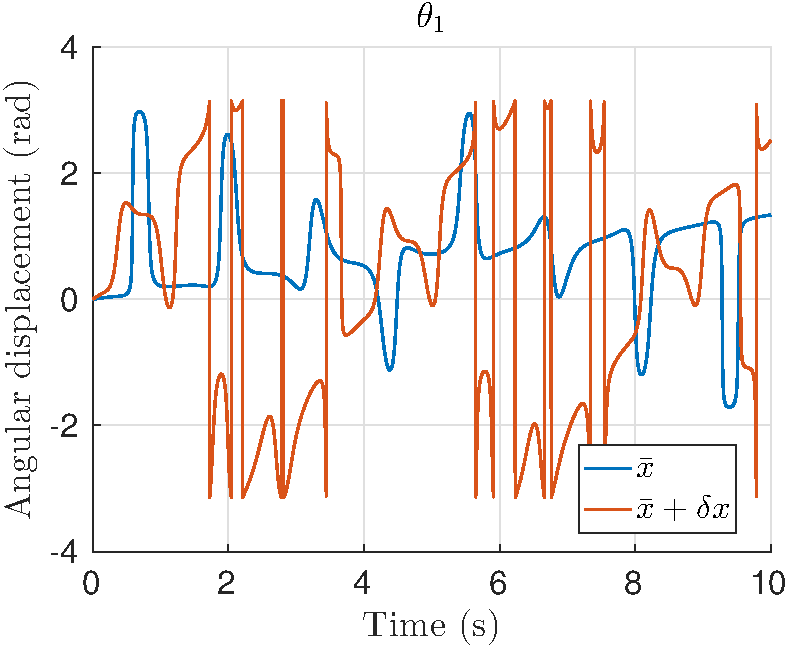
\includegraphics[width=\columnwidth]{obs_dtheta1}
    \end{column}
    \begin{column}{0.37\textwidth}
      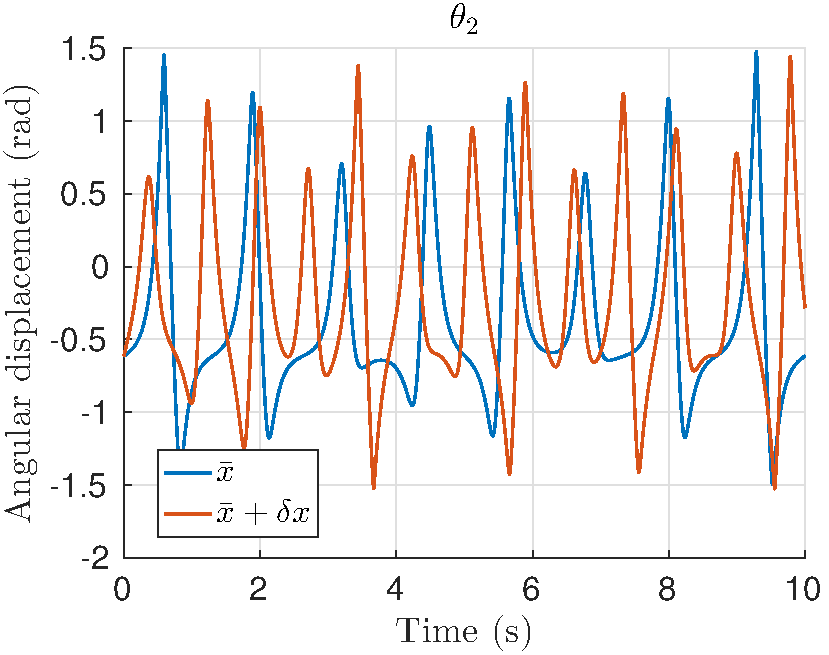
\includegraphics[width=\columnwidth]{obs_dtheta2}
    \end{column}
    \begin{column}{0.37\textwidth}
      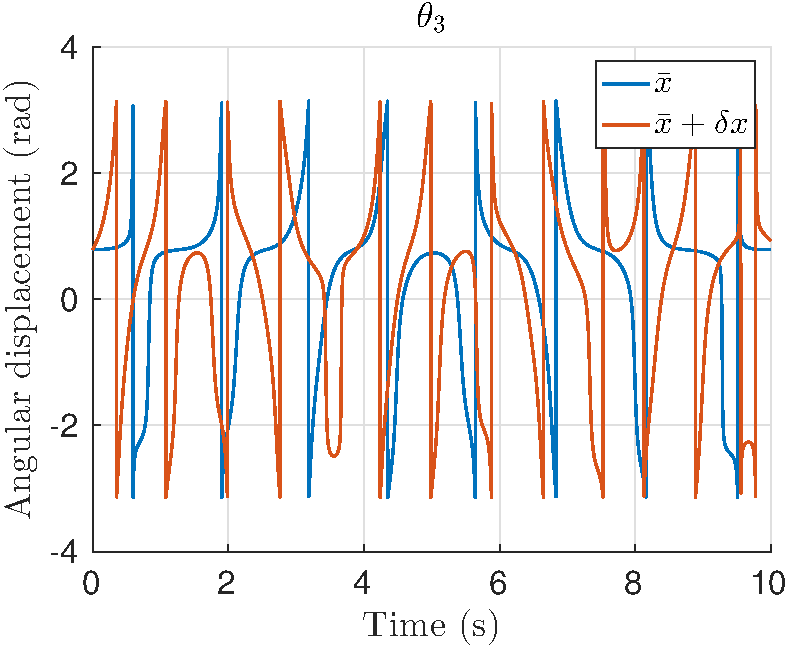
\includegraphics[width=\columnwidth]{obs_dtheta3}
    \end{column}
  \end{columns}
\end{frame}

\begin{frame}{Example 2 \cubli}
  Consider the initial state 
  \[
  \bar{\vec{x}} = 
  \begin{bmatrix}
    * & -\mathrm{atan}(\sqrt{2}/2) & \pi/4 & \bar{\dot{\vec{\theta}}} & 0 & 0 & 0
  \end{bmatrix}\transpose
  \]
  An initial state $\bar{\vec{x}} + \vec{\delta x}$ where
  \[
  \vec{\delta x} = \begin{bmatrix}
    0 & \hdots & \vec{\delta}\dot{\vec{q}}_{wheels}
  \end{bmatrix}\transpose
  \]
  produces a different output.
  \begin{columns}
    \begin{column}{0.37\textwidth}
      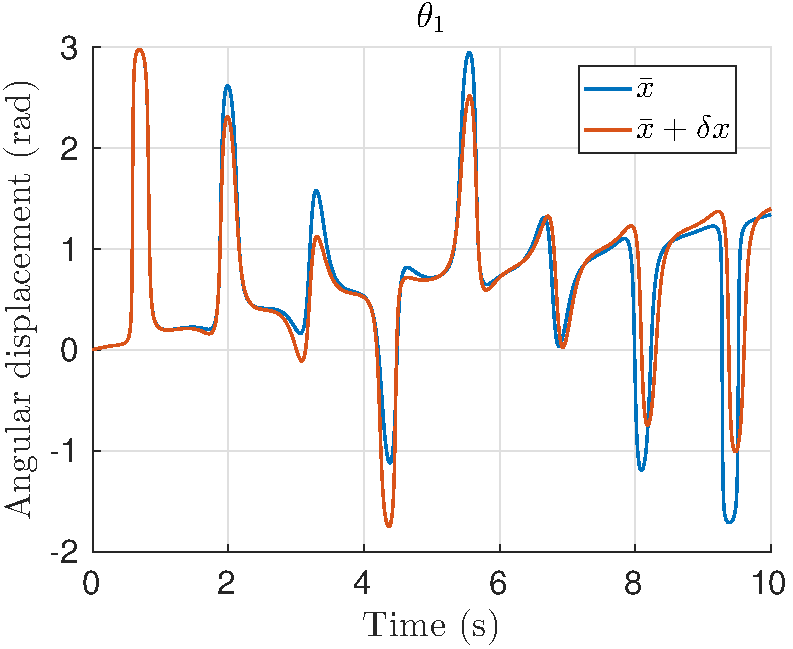
\includegraphics[width=\columnwidth]{obs_dq1}
    \end{column}
    \begin{column}{0.37\textwidth}
      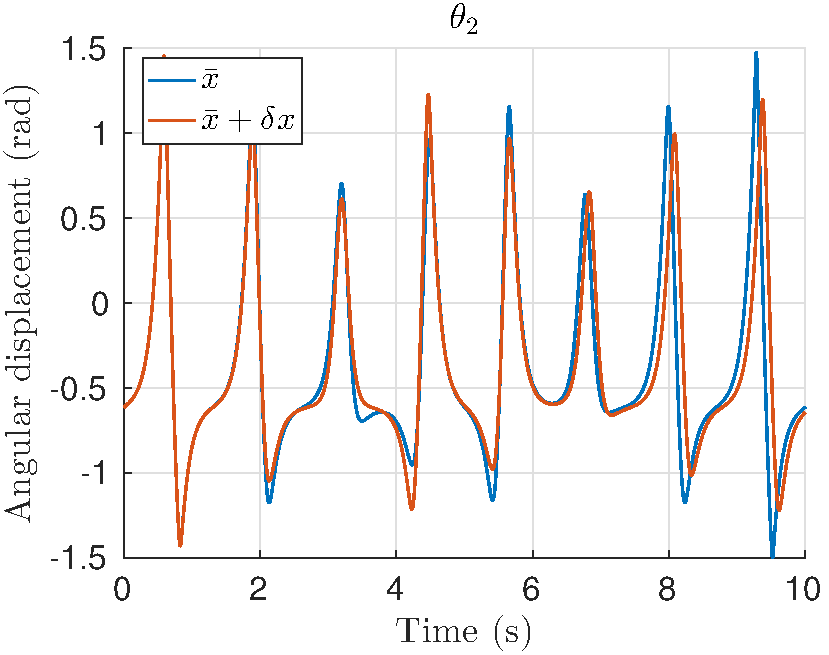
\includegraphics[width=\columnwidth]{obs_dq2}
    \end{column}
    \begin{column}{0.37\textwidth}
      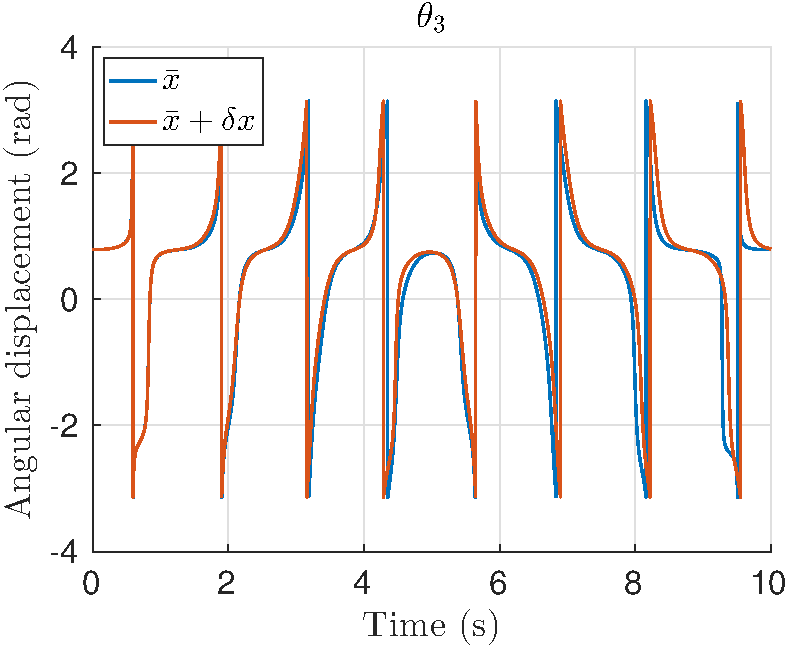
\includegraphics[width=\columnwidth]{obs_dq3}
    \end{column}
  \end{columns}
\end{frame}

\begin{frame}{Observability codistribution \cubli}
  \begin{exampleblock}{Observability codistribution for the Cubli \hfill $\bar{\vec{x}} \in \mathcal{E}_{1}$}
    Using the Symbolic Math Toolbox from MATLAB it turns out that for all $\bar{\vec{x}} \in \mathcal{E}_{1}$
    \[
    \mathrm{dim} (<\mathrm{\Delta} | d\vec{h}>) = 6 < n = 9
    \]
    but the codistribution is \alert{not} regular then the theorem \alert{cannot} be applied.
  \end{exampleblock}
\end{frame}
